

As shown in Figure \ref{fig:roib_summary}, the performance of the PC-RoIB with realistic running ATLAS conditions
is improved over the VME-RoIB particularly at high RoI sizes. 

\begin{figure}[t!]
\centering
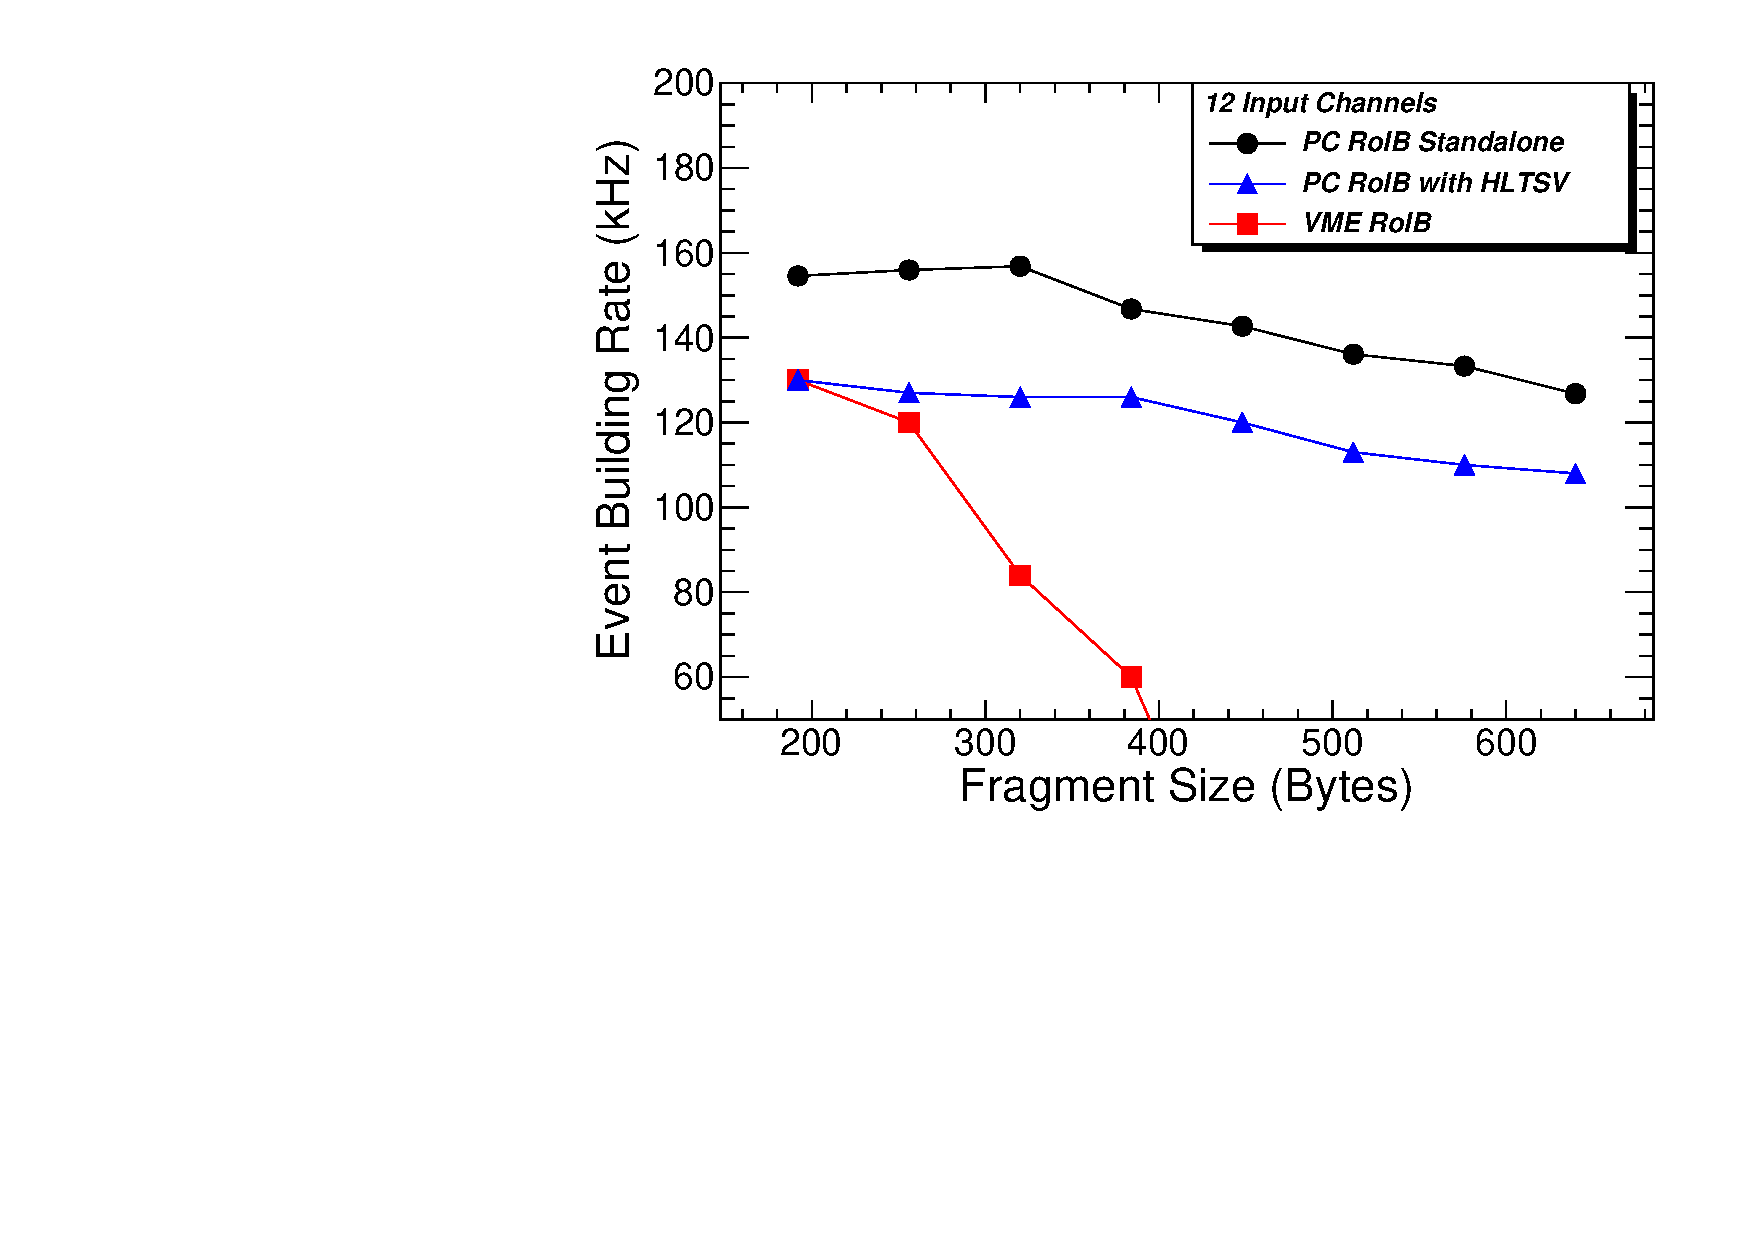
\includegraphics[width=0.5\textwidth]{roib_summary_size} 
\caption{The event building rate as a function of the RoI record size in Bytes. The rates are shown for a standalone application that implements 
a minimal interface for event building, the integrated RoIB software into an HLTSV process
running within the full ATLAS TDAQ software suite, and for comparison the VME-RoIB performance.}
\label{fig:roib_summary}
\end{figure} 

\begin{figure}[p!]
\centering
 \begin{subfigure}{0.48\textwidth}
 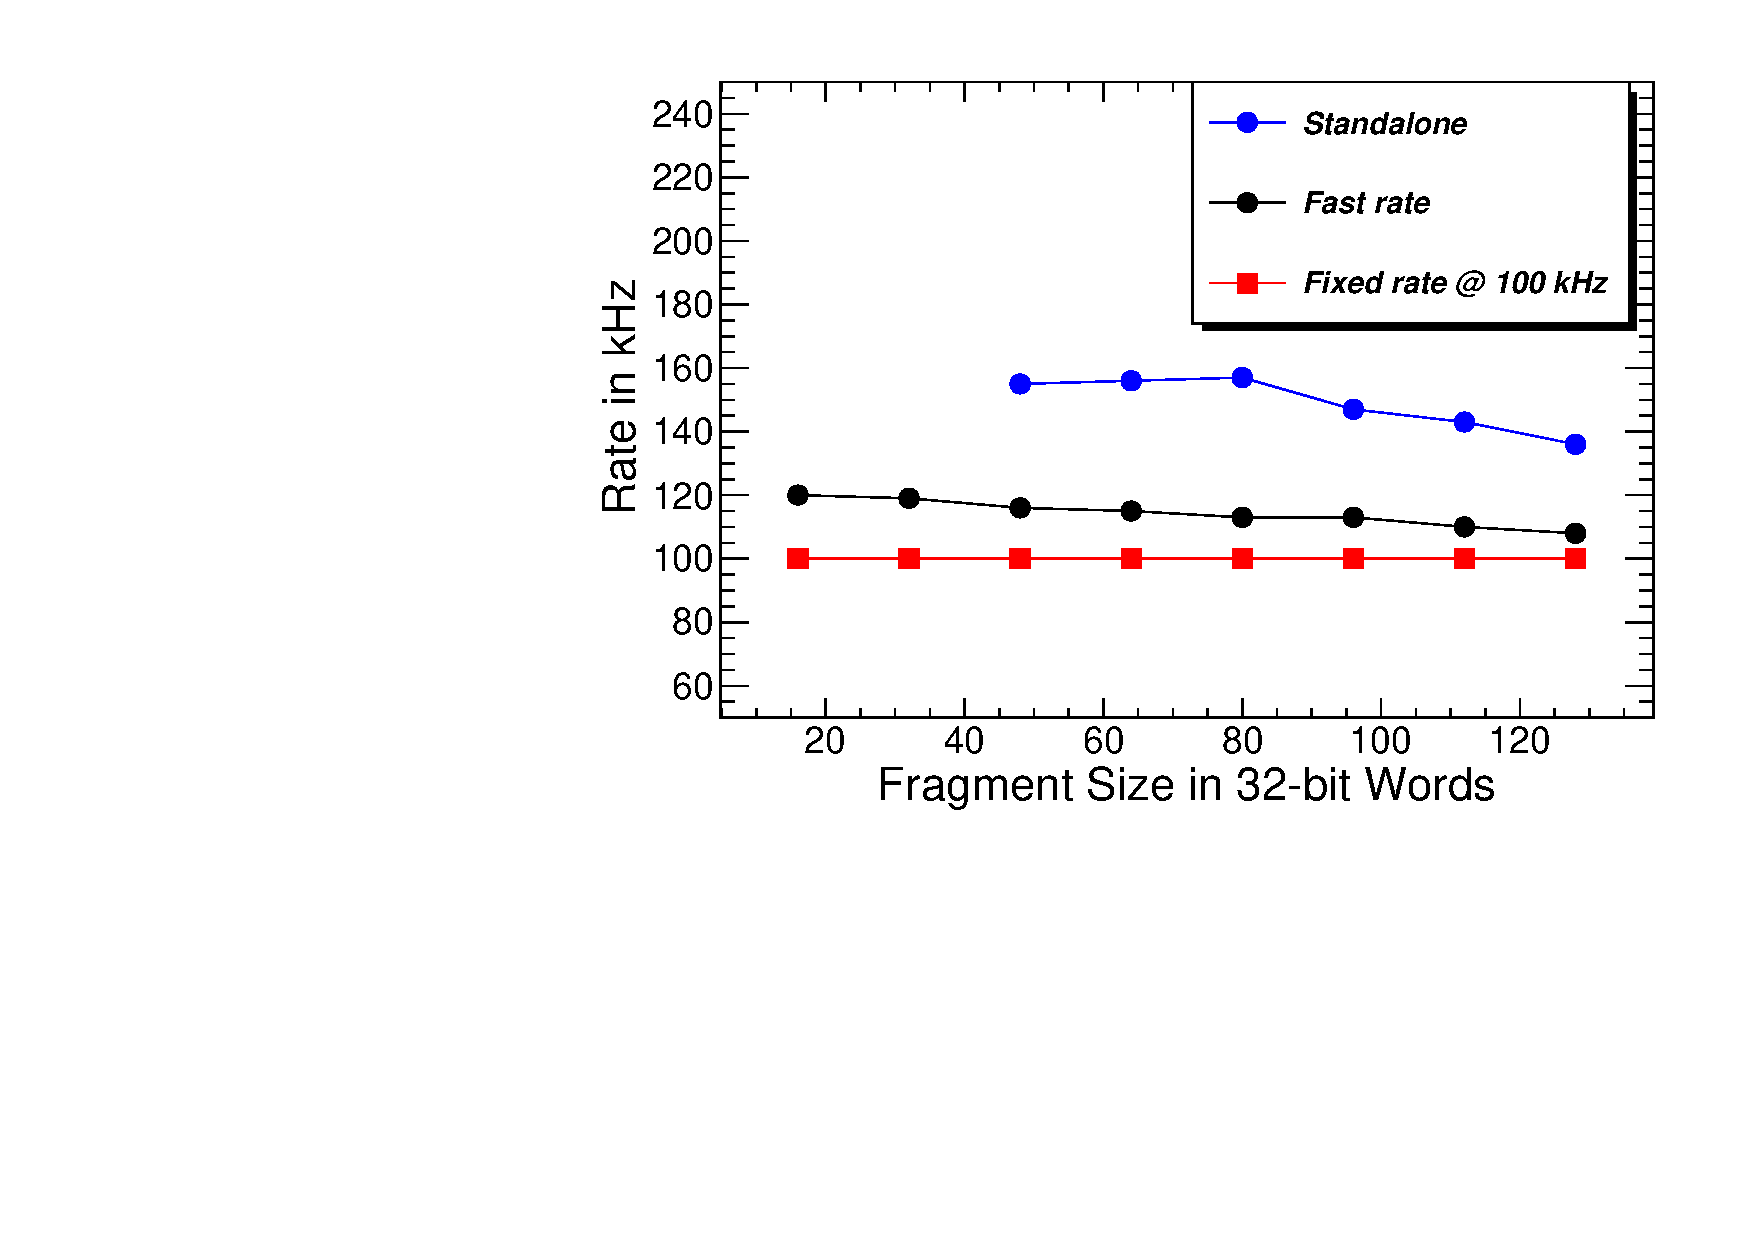
\includegraphics[width=\textwidth]{rate_final}
 \subcaption{}
 \end{subfigure}
 \begin{subfigure}{0.48\textwidth}
 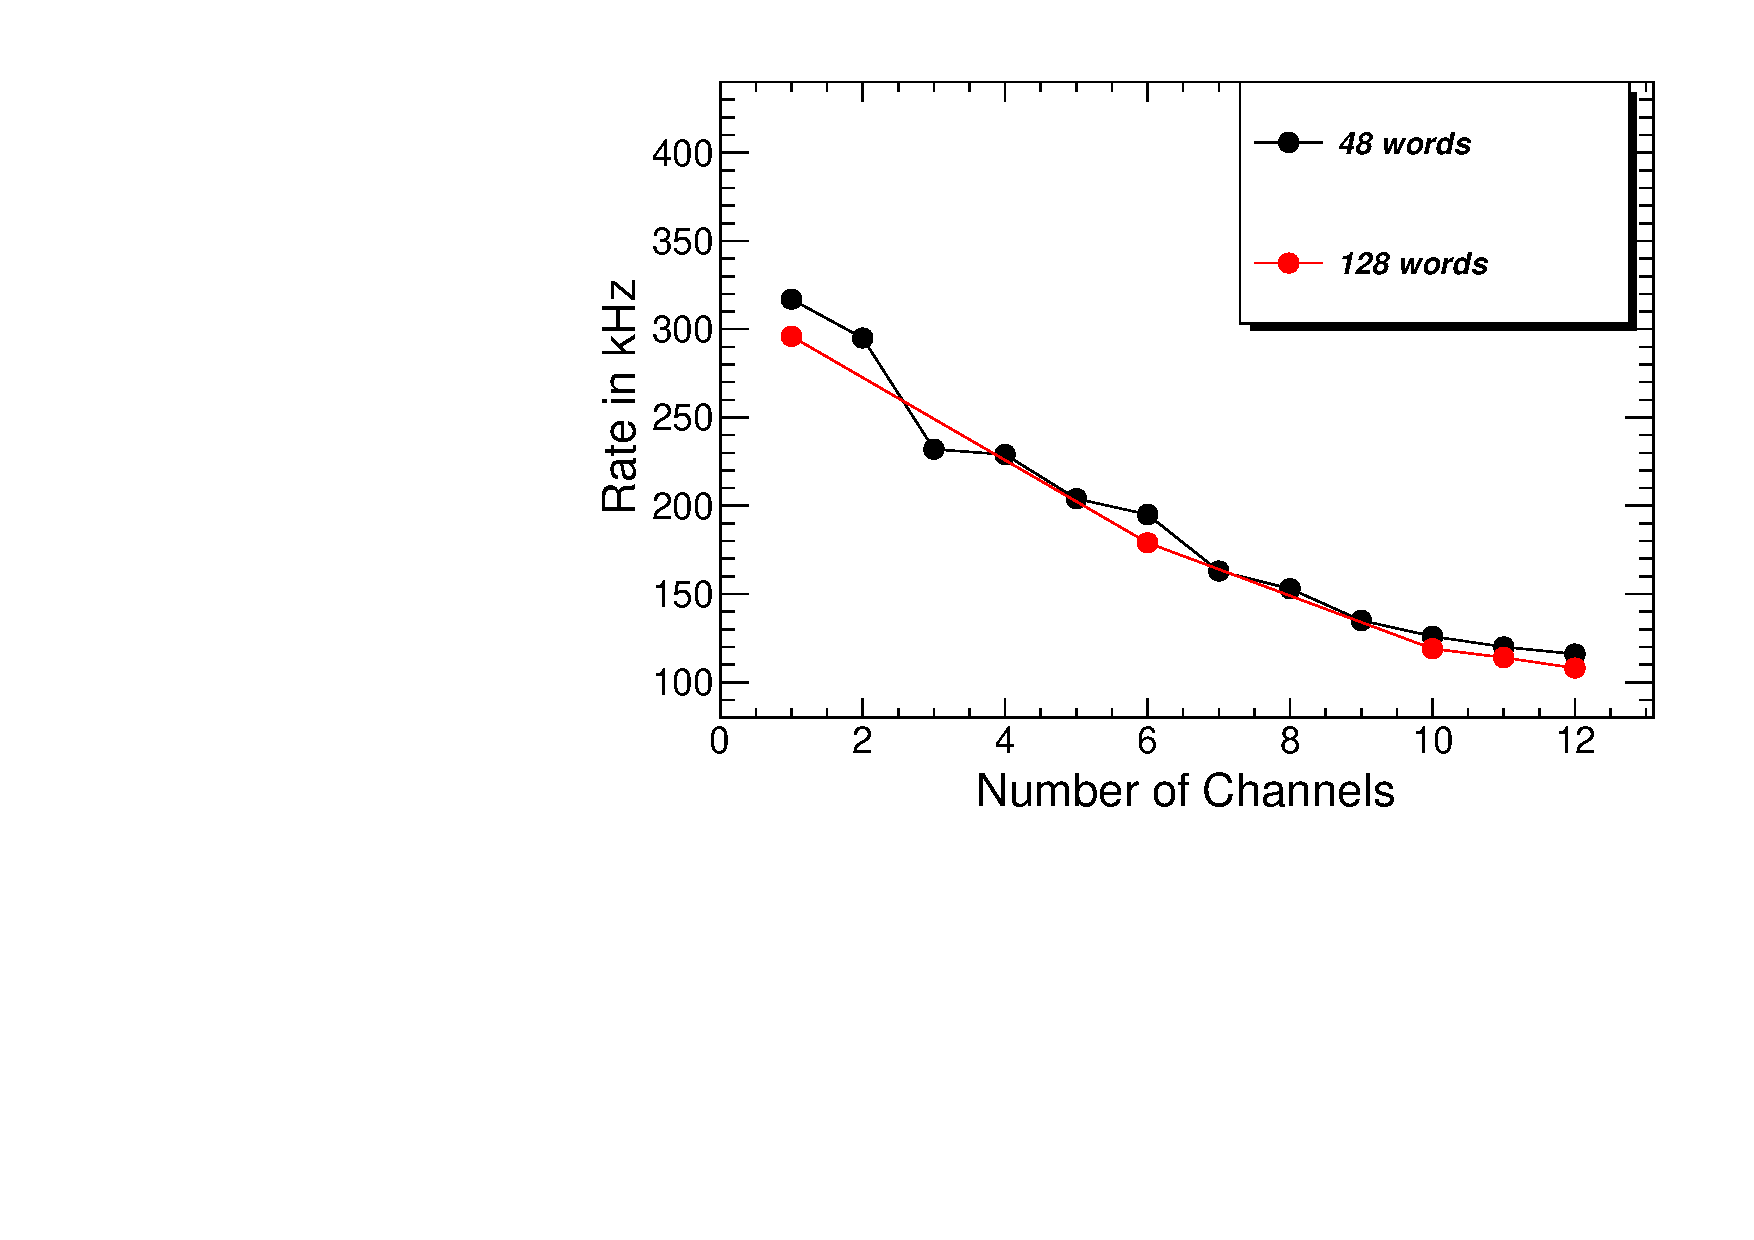
\includegraphics[width=\textwidth]{channel_tests}
 \subcaption{}
 \end{subfigure}
   \caption{
}
\label{fig:roib.perf.other}
\end{figure}

Figure \ref{fig:roib_pileup_l1rate} shows that the memory usage of the HLTSV is at the level of 5\% and that the RoIB event assembly does not depend 
on pileup conditions.


\begin{figure}[t!]
\centering
\begin{subfigure}[t]{0.48\textwidth}
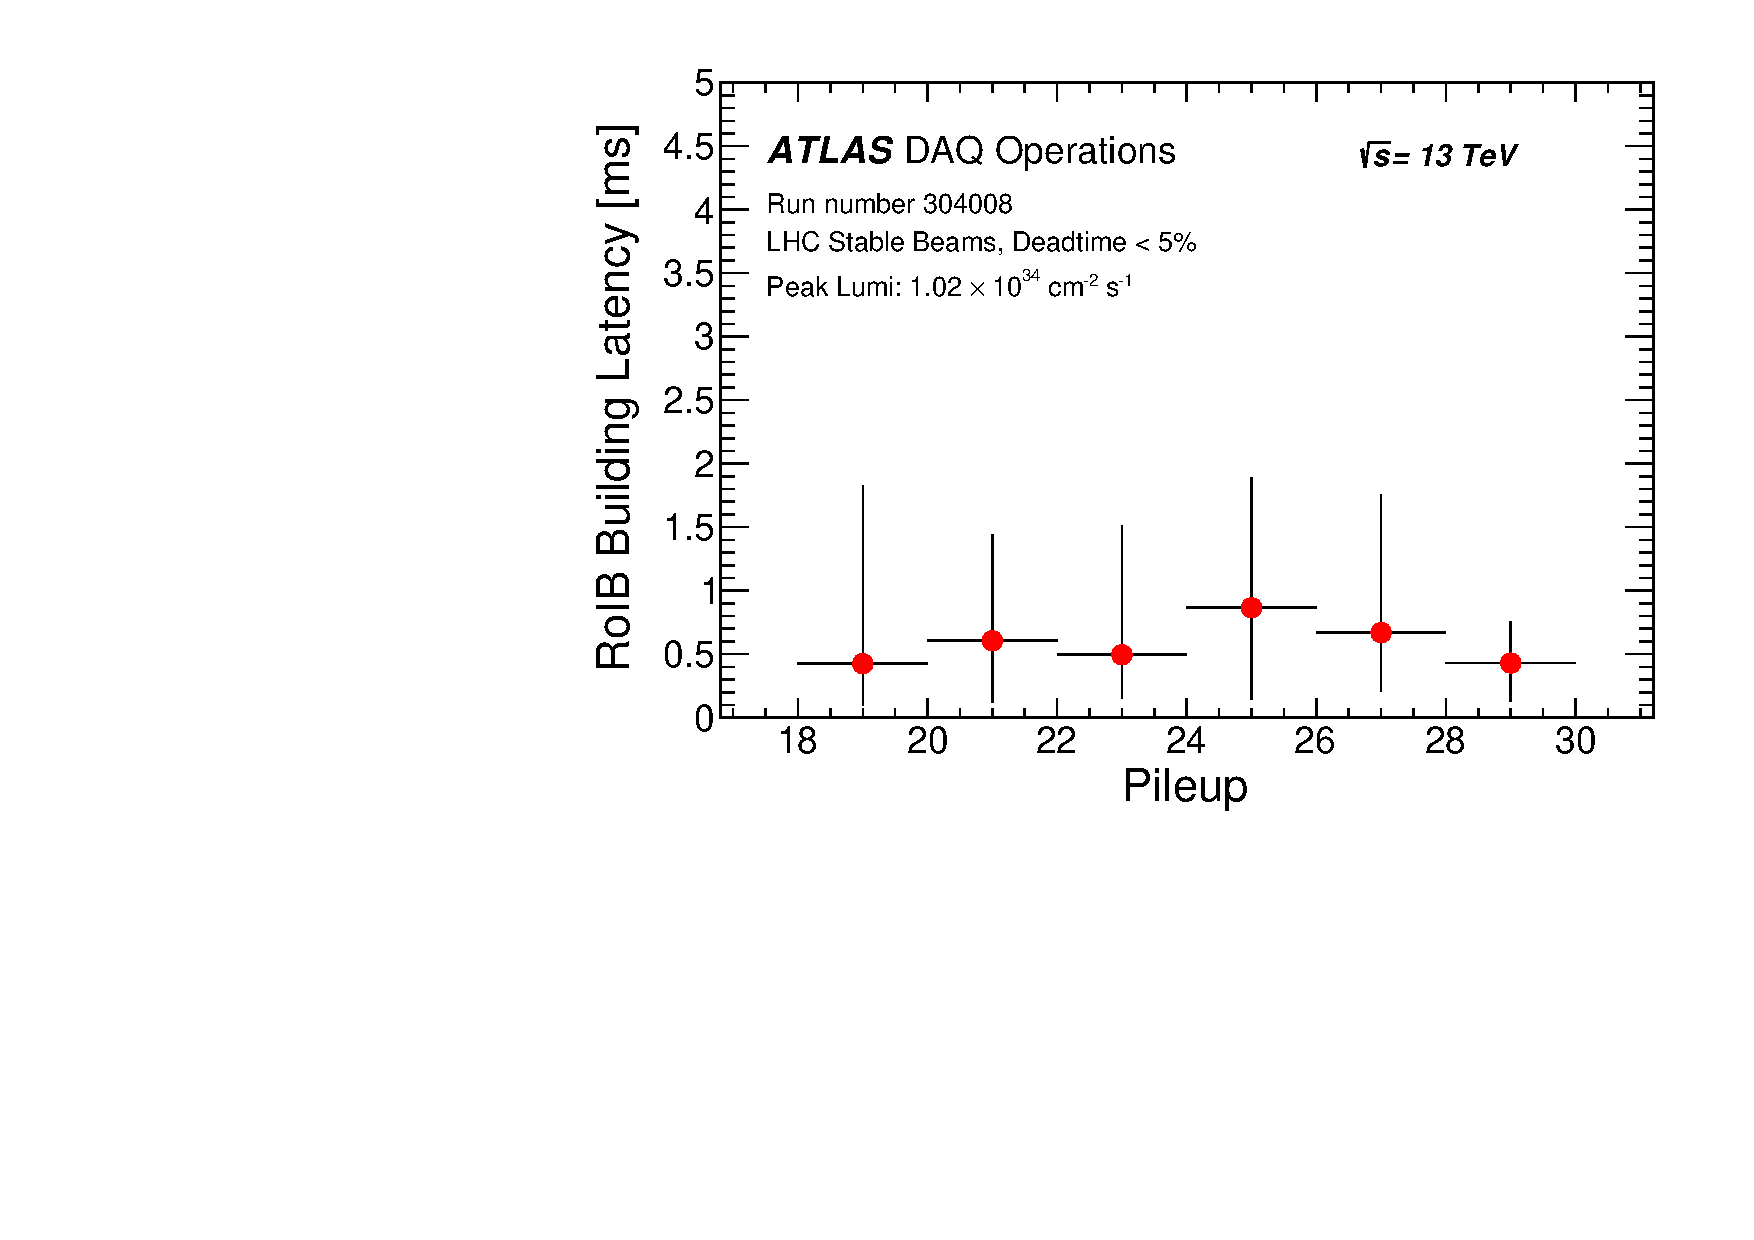
\includegraphics[width=0.95\textwidth]{GrAssym_run_304008_pileup_RoIBbuildtime}
\end{subfigure}
\begin{subfigure}[t]{0.48\textwidth}
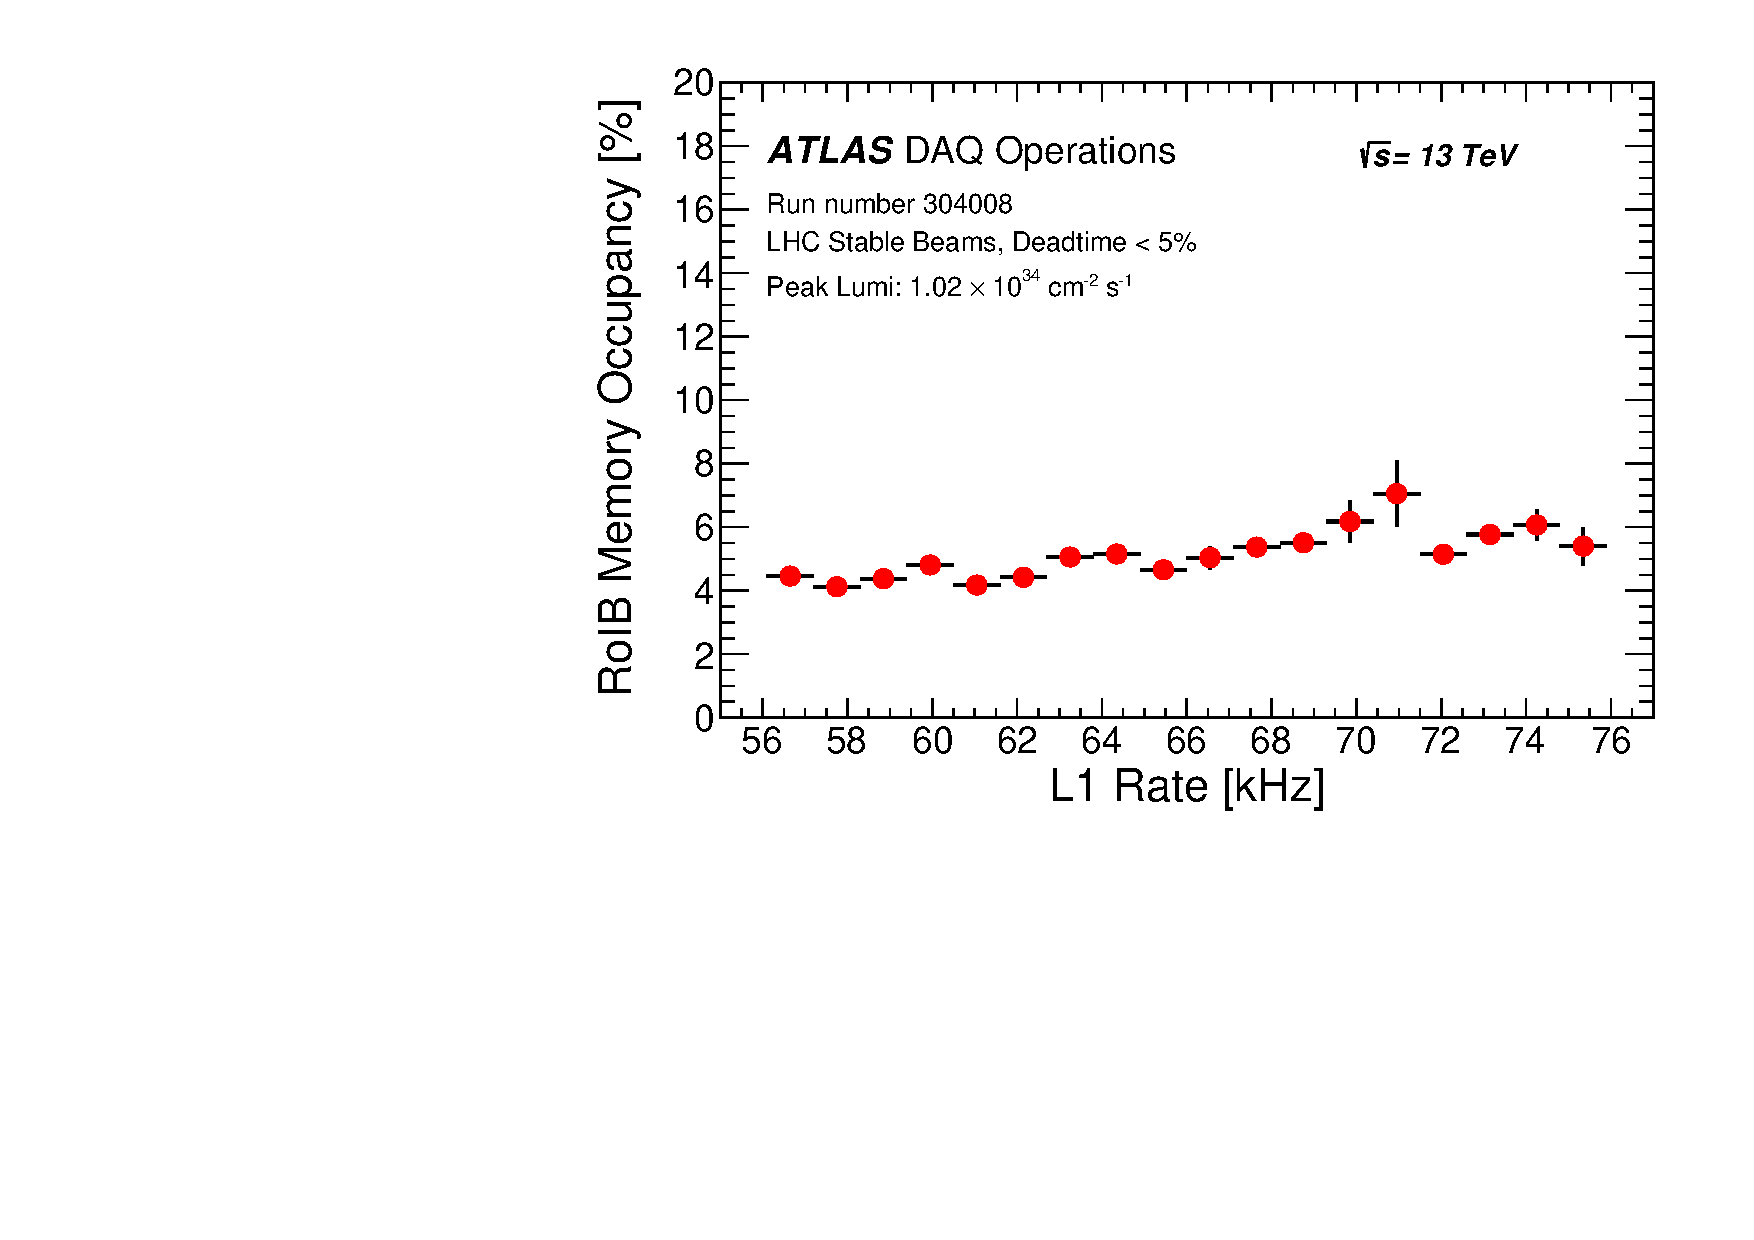
\includegraphics[width=0.95\textwidth]{hProf_run_304008_l1rate_RoIBMemOccup}
\end{subfigure}
\vspace{-0.25cm}
\caption{RoIB performance: RoIB building latency as a function of pileup (left), RoIB memory occupancy as a function of L1 rate (right).}
\label{fig:roib_pileup_l1rate}
\end{figure} 




\begin{figure}[t!]
\centering
\begin{subfigure}[t]{0.48\textwidth}
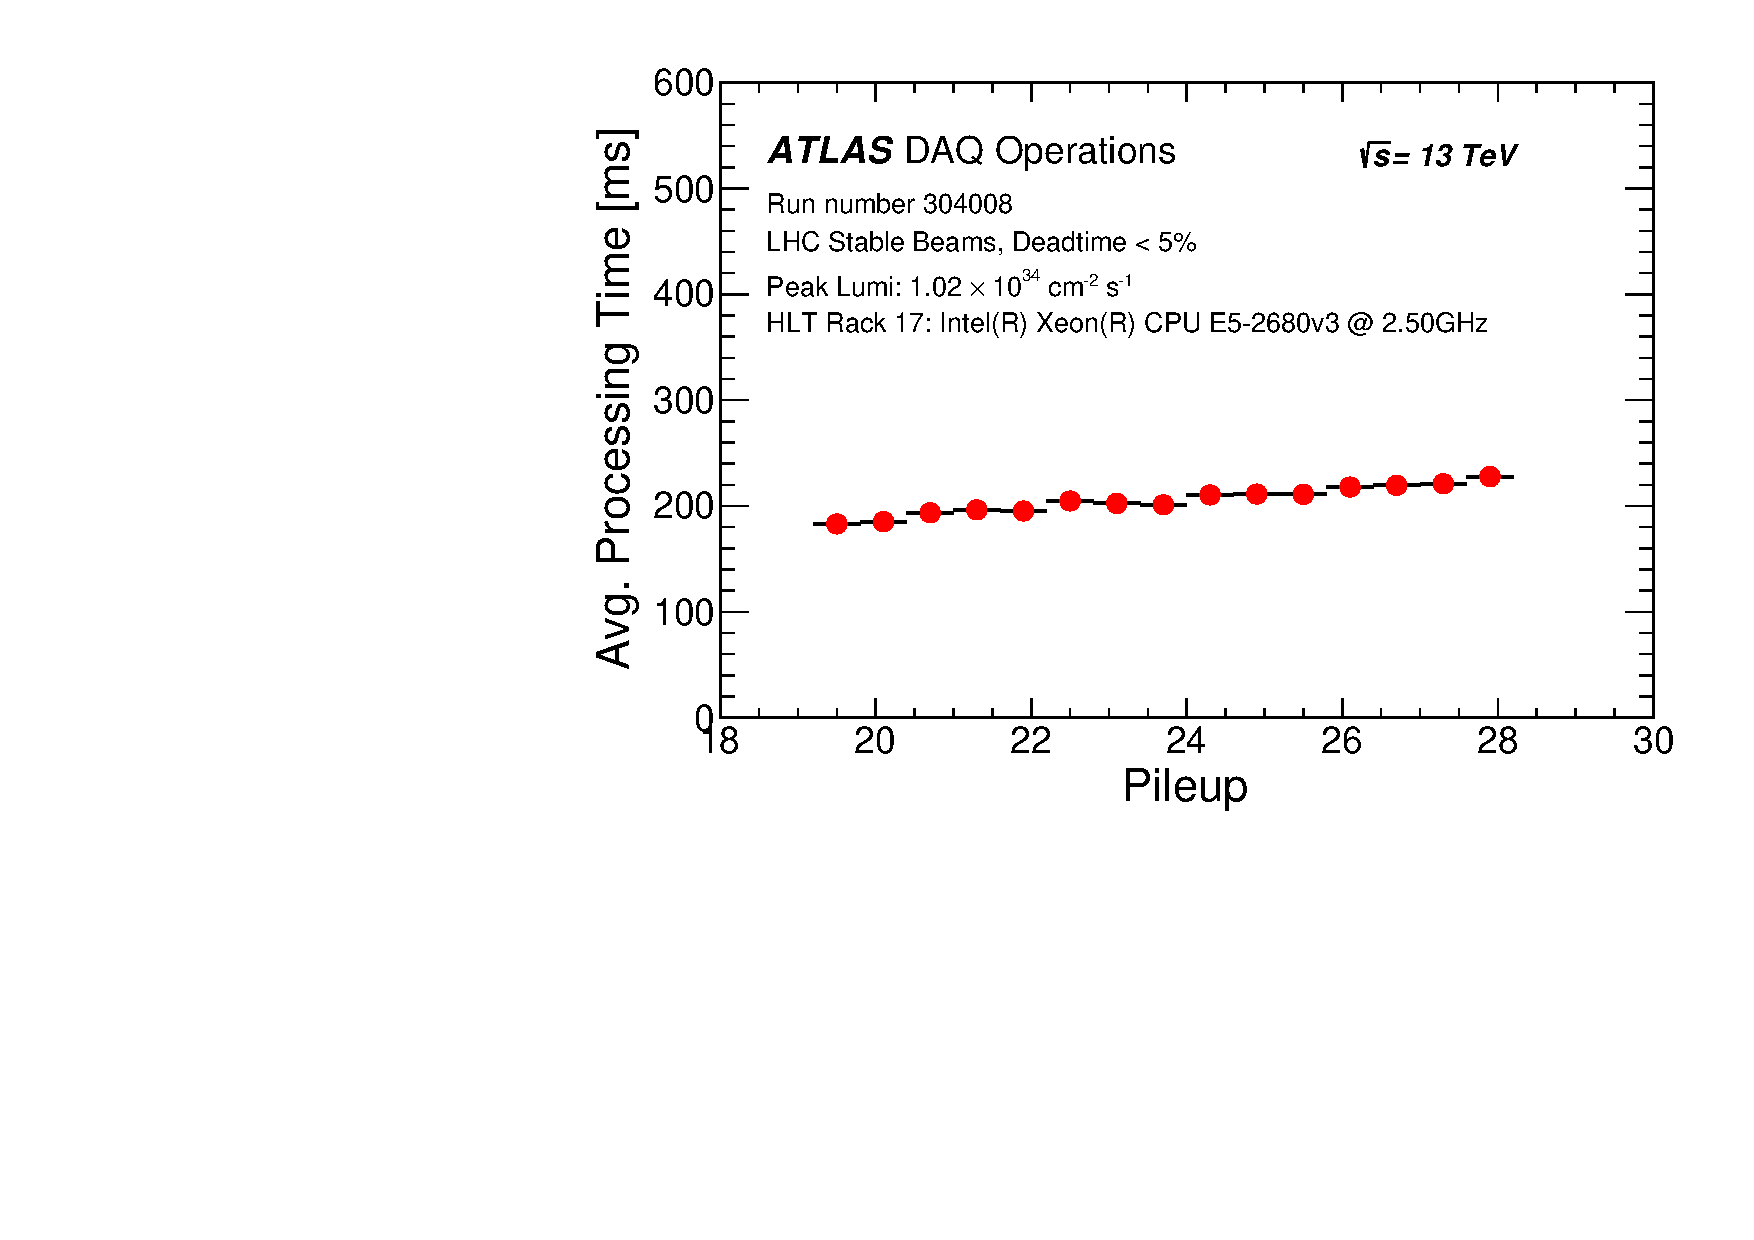
\includegraphics[width=0.95\textwidth]{hProf_run_304008_pileup_AvgProcessingTime}
\end{subfigure}
\begin{subfigure}[t]{0.48\textwidth}
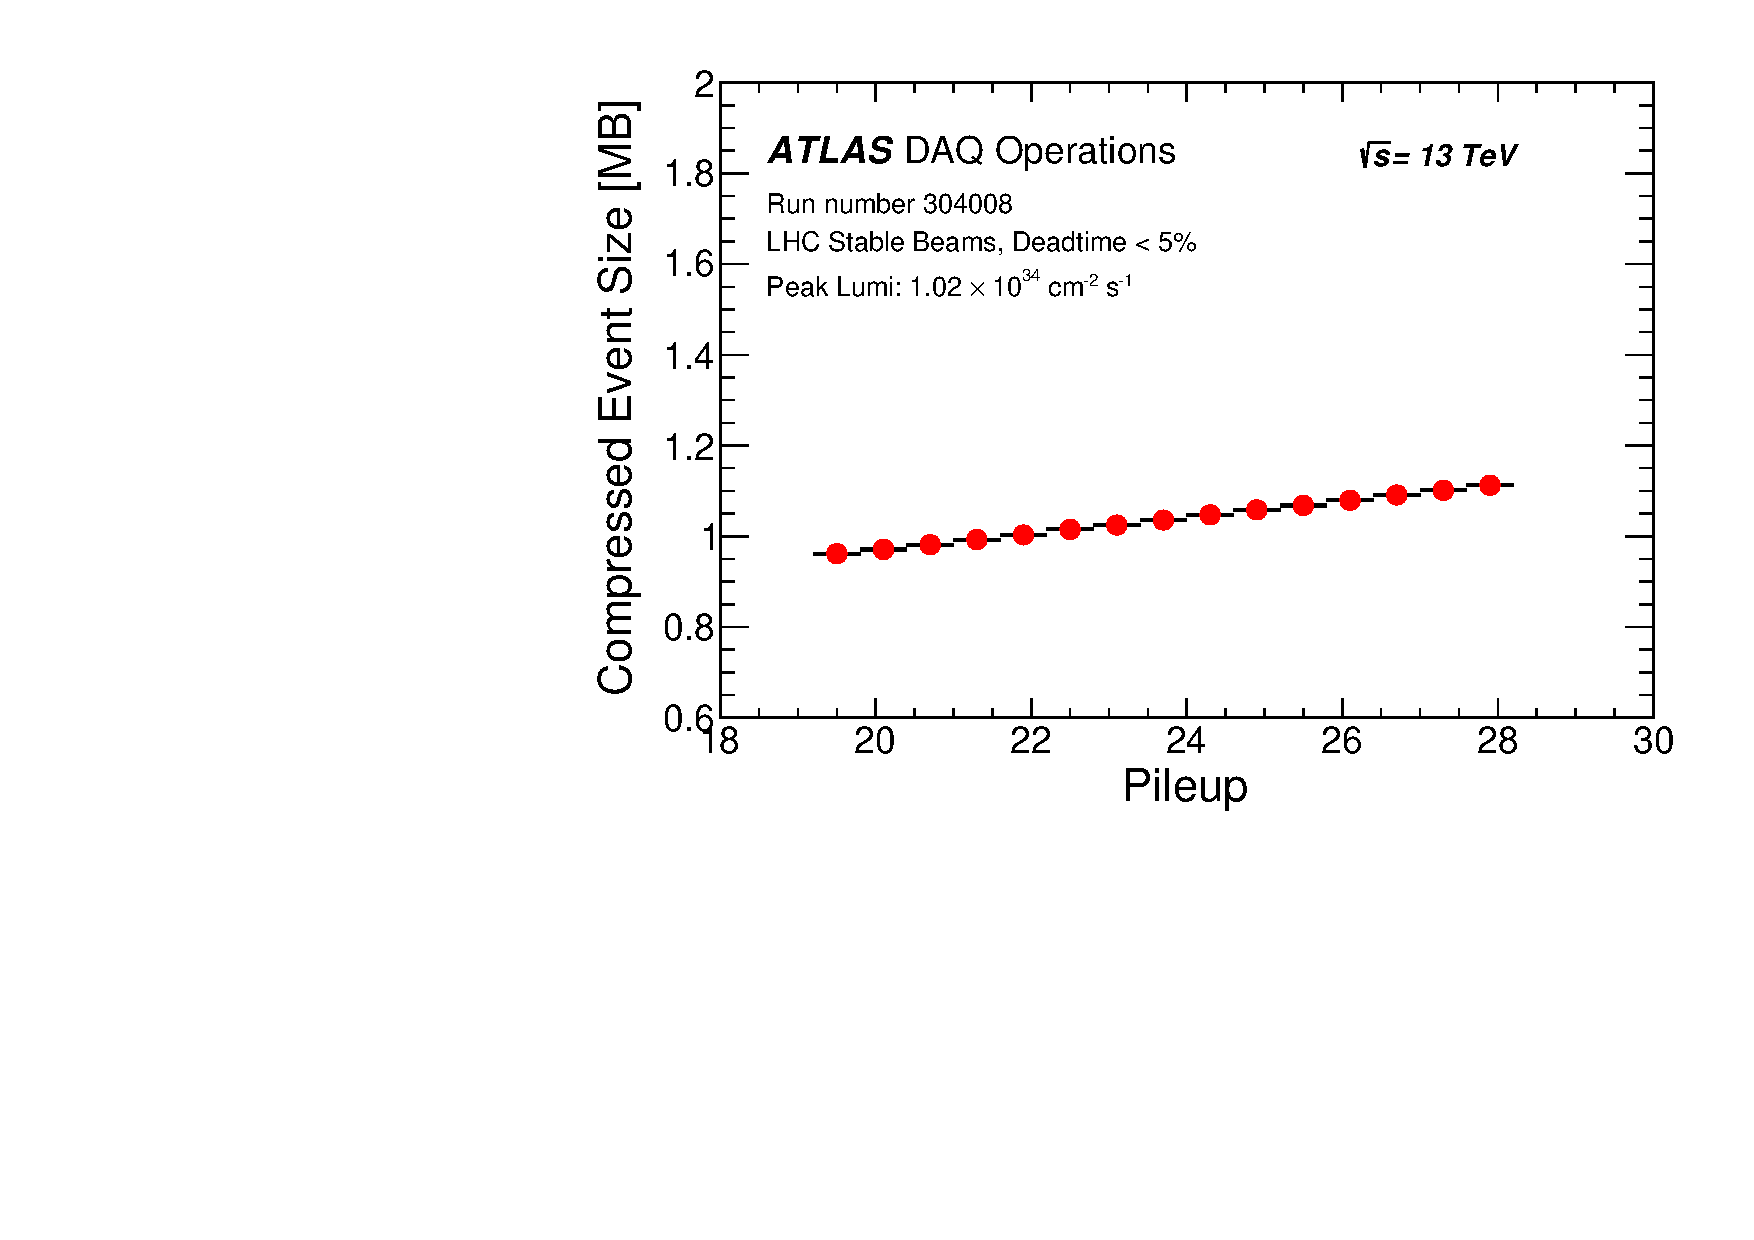
\includegraphics[width=0.95\textwidth]{hProf_run_304008_pileup_EventSize}
\end{subfigure}
\vspace{-0.25cm}
\caption{}
\label{fig:}
\end{figure} 
